\documentclass[]{article}
\usepackage{lmodern}
\usepackage{amssymb,amsmath}
\usepackage{ifxetex,ifluatex}
\usepackage{fixltx2e} % provides \textsubscript
\ifnum 0\ifxetex 1\fi\ifluatex 1\fi=0 % if pdftex
  \usepackage[T1]{fontenc}
  \usepackage[utf8]{inputenc}
\else % if luatex or xelatex
  \ifxetex
    \usepackage{mathspec}
  \else
    \usepackage{fontspec}
  \fi
  \defaultfontfeatures{Ligatures=TeX,Scale=MatchLowercase}
\fi
% use upquote if available, for straight quotes in verbatim environments
\IfFileExists{upquote.sty}{\usepackage{upquote}}{}
% use microtype if available
\IfFileExists{microtype.sty}{%
\usepackage{microtype}
\UseMicrotypeSet[protrusion]{basicmath} % disable protrusion for tt fonts
}{}
\usepackage{hyperref}
\hypersetup{unicode=true,
            pdftitle={Network based multifactorial modelling microRNA-target interaction.},
            pdfauthor={Selcen Ari; Alper Yilmaz},
            pdfborder={0 0 0},
            breaklinks=true}
\urlstyle{same}  % don't use monospace font for urls
\usepackage{graphicx,grffile}
\makeatletter
\def\maxwidth{\ifdim\Gin@nat@width>\linewidth\linewidth\else\Gin@nat@width\fi}
\def\maxheight{\ifdim\Gin@nat@height>\textheight\textheight\else\Gin@nat@height\fi}
\makeatother
% Scale images if necessary, so that they will not overflow the page
% margins by default, and it is still possible to overwrite the defaults
% using explicit options in \includegraphics[width, height, ...]{}
\setkeys{Gin}{width=\maxwidth,height=\maxheight,keepaspectratio}
\IfFileExists{parskip.sty}{%
\usepackage{parskip}
}{% else
\setlength{\parindent}{0pt}
\setlength{\parskip}{6pt plus 2pt minus 1pt}
}
\setlength{\emergencystretch}{3em}  % prevent overfull lines
\providecommand{\tightlist}{%
  \setlength{\itemsep}{0pt}\setlength{\parskip}{0pt}}
\setcounter{secnumdepth}{0}
% Redefines (sub)paragraphs to behave more like sections
\ifx\paragraph\undefined\else
\let\oldparagraph\paragraph
\renewcommand{\paragraph}[1]{\oldparagraph{#1}\mbox{}}
\fi
\ifx\subparagraph\undefined\else
\let\oldsubparagraph\subparagraph
\renewcommand{\subparagraph}[1]{\oldsubparagraph{#1}\mbox{}}
\fi

%%% Use protect on footnotes to avoid problems with footnotes in titles
\let\rmarkdownfootnote\footnote%
\def\footnote{\protect\rmarkdownfootnote}

%%% Change title format to be more compact
\usepackage{titling}

% Create subtitle command for use in maketitle
\providecommand{\subtitle}[1]{
  \posttitle{
    \begin{center}\large#1\end{center}
    }
}

\setlength{\droptitle}{-2em}

  \title{Network based multifactorial modelling microRNA-target interaction.}
    \pretitle{\vspace{\droptitle}\centering\huge}
  \posttitle{\par}
    \author{Selcen Ari\footnote{Department of Bioengineering, Yildiz Technical
  University, Istanbul, Turkey} \\ Alper Yilmaz\footnote{Department of Bioengineering, Yildiz Technical
  University, Istanbul, Turkey}}
    \preauthor{\centering\large\emph}
  \postauthor{\par}
      \predate{\centering\large\emph}
  \postdate{\par}
    \date{10 Eylül 2019}


\begin{document}
\maketitle

\hypertarget{abstract}{%
\subsection{Abstract}\label{abstract}}

Competing endogenous RNA (ceRNA) regulations and crosstalk between
various types of non-coding RNA in human is remarkable in means of miRNA
regulation. Many studies have pointed out that an alteration in
miRNA:target interaction can result in unexpected changes due to
indirect and complex interactions. In this paper, we defined a new
network-based model that handles miRNA:ceRNA interactions with
expression values. Our model is able to handle miRNA interaction factors
such as seed type, binding energy, if provided. Our approach is able to
reveal that a perturbation in an element of network affects whole
competing elements differently and cooperative efficiencies of miRNAs on
common targets could be calculated. Our findings emphasized importance
of miRNA:target ratios being crucial, as reported by previous studies.
We have showed that the competing elements which have the same or close
expression values may not be affected equally from the perturbation
because of repression functionality depended on interaction factors of
miRNA target pairs (answer: Hocam etkileşim faktörlerinden dolayı
ekspresyonları yakın olsa bile baskılanma aktitesinin aynı
sergilenmeyeceğini ifade etmeye çalıştım. Bu şekilde anlaşılıyor mu?).
We applied the model to real sample consisting of breast cancer gene and
miRNA expression dataset and experimental miRNA:target interaction
dataset all generated via high throughput sequencing methods. A gene
over-expressed in tumor tissue, namely \emph{ABCC1}, is used as
perturbing element. We have observed that change in expression level of
single gene in miRNA:target network is sufficient to perturb regulations
in whole network, due to unforeseen and unpredicted regulation which are
only visible when considered in network context. Therefore, this model
helps unveiling the crosstalk between elements in miRNA:target network
where abundance of target and sponge effect are taken into account. The
model is scalable and can be plugged in with emerging miRNA effectors
such as circRNAs. The model is available as R package
\href{https://github.com/selcenari/ceRNAnetsim}{ceRNAnetsim}.

\hypertarget{introduction}{%
\subsection{Introduction}\label{introduction}}

MicroRNAs (miRNAs) are a family of short non-coding RNAs which are key
regulator of gene expression through various post-transcriptional
mechanisms. Although the mechanisms by which miRNA represses are not
fully understood, miRNAs predominantly repress their targets. Repressive
activities of miRNAs vary depending on many factors that are significant
to miRNA:target interactions. These factors include miRNA:target binding
energy, binding location in target sequence, base pairing types between
miRNA and target, abundance of miRNAs and targets (Grimson et al.
\protect\hyperlink{ref-grimson_microrna_2007}{2007}). Binding energies
of miRNA:target complexes vary based on nucleotide context and determine
folding stability of complex (Cao and Chen
\protect\hyperlink{ref-cao_predicting_2012}{2012}). It has been
demonstrated that the binding energy between miRNA and target indicates
stability or affinity of complex (Helwak et al.
\protect\hyperlink{ref-helwak_mapping_2013}{2013}) and does not directly
determine repressive activity of miRNA (Cao and Chen
\protect\hyperlink{ref-cao_predicting_2012}{2012}). Early studies have
argued that 2-8 nt sequence, seed, located in miRNA 5'end bind to
specific sequence located in 3'UTR of its target (Bartel
\protect\hyperlink{ref-bartel_micrornas_2004}{2004}; Lewis, Burge, and
Bartel \protect\hyperlink{ref-lewis_conserved_2005}{2005}). In recent
studies, it has been shown that miRNAs can interact with targets via
sequences located in regions such as 5'UTR or CDS (Hausser et al.
\protect\hyperlink{ref-hausser_analysis_2013}{2013}; Helwak et al.
\protect\hyperlink{ref-helwak_mapping_2013}{2013}; Moore et al.
\protect\hyperlink{ref-moore_mirnatarget_2015}{2015}). These studies
also showed that binding location could indicate functionality of
miRNA:target interaction or be effective on abundance of targets(TOFIX
abundance etkisi derken, bazen azaltabilir, bazen arttırabilir,
manasında mı? answer: evet hocam anlaşılmıyorsa değiştirebilirim). It
has been shown that miRNAs exhibit repressive activity via, 6-8 nt long
sequence that is perfectly complementary with targets, seed region at
the 5' end of miRNAs (Bartel
\protect\hyperlink{ref-bartel_micrornas:_2009}{2009}; Grimson et al.
\protect\hyperlink{ref-grimson_microrna_2007}{2007}). On the other hand,
some researchers have reported that seed sequence of miRNA can have
mismatches or bulged/wobble nucleotides (Chi, Hannon, and Darnell
\protect\hyperlink{ref-chi2012alternative}{2012}) and may locate in
region other than 5'end of miRNAs (Hafner et al.
\protect\hyperlink{ref-hafner_transcriptome-wide_2010}{2010}; Helwak et
al. \protect\hyperlink{ref-helwak_mapping_2013}{2013}). On top of all
these factors, abundance of miRNAs and targets and miRNA:target ratio in
cells predominantly affect efficiency of miRNA:target interaction (Arvey
et al. \protect\hyperlink{ref-arvey_target_2010}{2010}; Bosson, Zamudio,
and Sharp \protect\hyperlink{ref-bosson_endogenous_2014}{2014}; Denzler
et al. \protect\hyperlink{ref-denzler_assessing_2014}{2014}).

As it is possible for miRNAs to suppress multiple targets, an individual
mRNA molecule can also be targeted by multiple miRNAs. In that case, the
targeted mRNAs exhibit competitor behavior, that is hypothesized as
competing endogenous RNAs (ceRNAs) (Ala et al.
\protect\hyperlink{ref-ala_integrated_2013}{2013}; Cesana and Daley
\protect\hyperlink{ref-cesana_deciphering_2013}{2013}), against their
miRNAs. Briefly, Ala et al.~have explained the ceRNA hypothesis as
disturbance of the other target when one of the targets on a
steady-state system that included one miRNA and two target was perturbed
with expression change (Ala et al.
\protect\hyperlink{ref-ala_integrated_2013}{2013}). Regarding
interaction between miRNAs and their target in a cell, explaining and
predicting results of an individual perturbation is difficult due to
complexity of interactions. Various computational and experimental
studies have tackled the problem of unraveling ceRNA:miRNA interactions.
It has been observed that when abundance of one of the targets of
miR-122 was increased, the other targets' expression also slightly
increased as a result of decreasing repressive activity of miR-122 on
them (Denzler et al.
\protect\hyperlink{ref-denzler_assessing_2014}{2014}). Bosson et
al.~have developed a mathematical model for changes on total target pool
concentration after grouping targets according to affinity and
demonstrated that miRNA activity correlated with affinity between miRNA
and target (Bosson, Zamudio, and Sharp
\protect\hyperlink{ref-bosson_endogenous_2014}{2014}). Cooperative
efficiency of miRNAs as well as competitor behaviors of targets were
also studied and it has been demonstrated to be crucial for regulating
available mRNA levels of targets (Denzler et al.
\protect\hyperlink{ref-denzler_impact_2016}{2016}). MiRNA:target
interactions have been modeled as stoichiometric and catalytic
mechanisms and Figliuzzi et al.~have recommended handling models in
network context (Figliuzzi, Marinari, and De Martino
\protect\hyperlink{ref-figliuzzi_micrornas_2013}{2013}). The model that
can explain miRNA target interaction through topological features has
been applied at bipartite network by Nitzan et al.~(Nitzan et al.
\protect\hyperlink{ref-nitzan_interactions_2014}{2014}). Robinson and
Henderson applied the model that handles miRNA:target direct and
indirect interactions via common targeting miRNA of genes and target of
miRNAs, at bipartite network. It has been demonstrated that all miRNAs
and targets in the network can interact with each other through common
miRNAs and genes, without interaction between the same type of nodes
(Robinson and Henderson
\protect\hyperlink{ref-robinson_modelling_2018}{2018}).Associated genes
that are targets of the same miRNAs have been found with help of
correlation of gene expression changes in recent algorithm (Markus List
\protect\hyperlink{ref-markus_list_sponge_2017}{2017}). List et al.~have
specified that their approach can be useful for ceRNA studies and
published their approach as an R package.

\hypertarget{methods}{%
\subsection{Methods}\label{methods}}

\hypertarget{construction-of-mirnatarget-network}{%
\subsubsection{Construction of miRNA:target
network}\label{construction-of-mirnatarget-network}}

miRNA and target pairs per line should be provided as edge list to
construct the network. At each line minimum required information is
expression levels of miRNA and the target. If available, additional data
about factors effecting binding or efficiency of miRNA can be provided
as separate columns. After construction of the network, amount of miRNA
per target is calculated and kept as edge data. Simply, a target will
sequester miRNA proportional to its ratio amount among other targets. If
additional criteria effecting the binding of miRNA to its target is
provided, distribution of miRNA will be calculated accordingly. Target
can be mRNA or any other ceRNA (circRNA, ncRNA, etc.) thus, throughout
the manuscript terms target, gene and ceRNA are used interchangeably.

\hypertarget{triggering-perturbation-and-subsequent-calculations}{%
\subsubsection{Triggering perturbation and subsequent
calculations}\label{triggering-perturbation-and-subsequent-calculations}}

Initially, the network is assumed in steady-state (\autoref{fig1}a)
condition and needs least one trigger for initiating calculations. The
trigger can be a change in expression level of one or more genes
(\autoref{fig1}b). After a trigger, the network undergoes iterative
cycle of calculations at each of which distribution of miRNA in local
neighborhood is recalculated (\autoref{fig1}c). Based on new miRNA
distribution, expression level of each node (i.e.~ceRNA) is updated.
This update results in change of expression value of common target (G4)
in system. In this case, the common target acts as trigger for the other
group (the targets interacted with M2 miRNA) in the network. Due to
common targeted elements, the change in one neighborhood spreads to
other neighborhoods (\autoref{fig1}d), consequently have potential to
effect whole network due to ``ripple effect''.

\begin{figure}
\hypertarget{fig1}{%
\centering
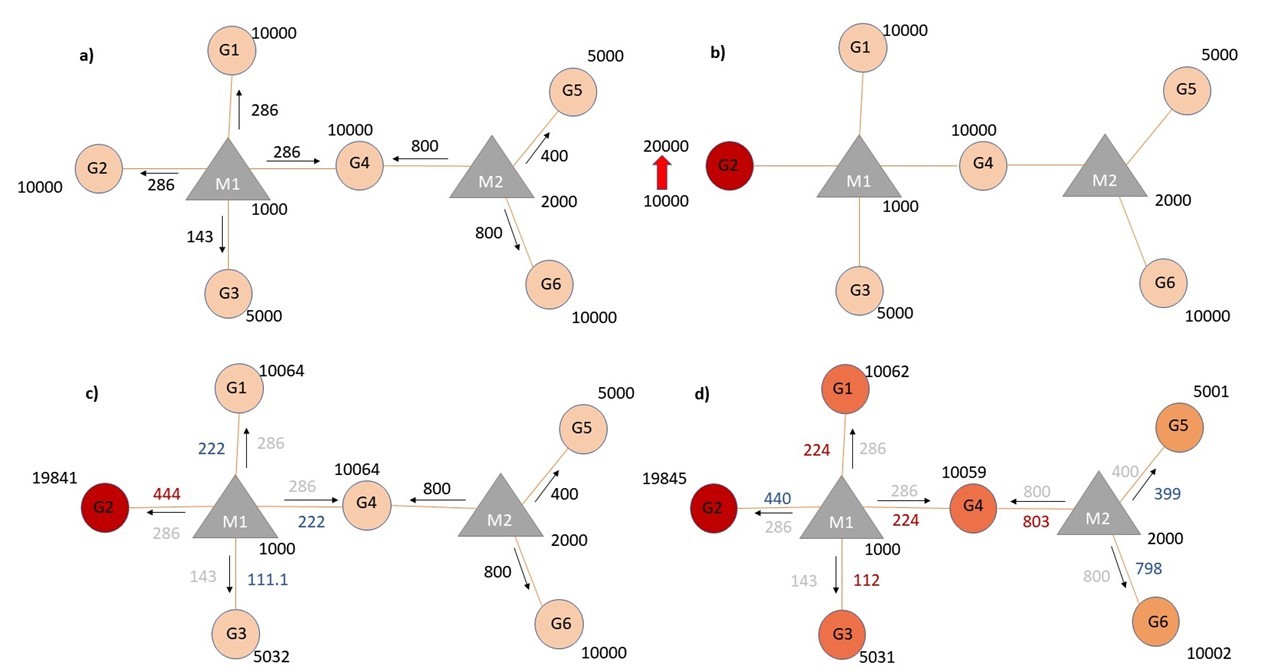
\includegraphics{Fig1.jpg}
\caption{Schematic presentation of mechanism of network based model. a)
In steady state, miRNAs (M: gray triangle) repress targets (G: circle
coconut) according to proportion of their targets' expression. b) Two
fold increase in transcript level of Gene2 (G2) acts as a trigger (shown
with red in figure). c) Distribution of miRNA1 (M1) changes. d) The
change at expression (shown with light red because minor changes are
occured on their expression values.) of common target effects changes of
proportional distribution of miRNA2 (M2). Expression values are rounded
to integers for simplicity}\label{fig1}
}
\end{figure}

During calculations, following assumptions were adopted; 1)
Transcription and degradation rates of miRNAs are steady and equal. 2)
All available miRNAs are recycled as in miRNA:ceRNA binding, target is
degraded and miRNA is unaffected. 3) ceRNA targets also have stable
transcription and degradation rates and these rates are equal.

The repression efficiency of a miRNA on the individual target
(\(Eff_{gi}\)) is calculated according to equation \eqref{eq:1}; where
miRNA expression (\(C_m\)) in local neighborhood is distributed among
targets using individual gene expression levels (\(C_{gi}\)) (\#FIX
isn't \(C_g\) gene expressions in the group is equal to total of
\(C_{gi}\) in group? answer: its my false. now its corect.). For the
genes targeted by multiple miRNAs, cooperative activity of miRNAs on a
target gene, \(R\), is calculated by summing repression activity of each
miRNA (Equation \eqref{eq:2}).

\begin{equation} 
    Eff_{gi}= C_m \times C_{gi}/\sum_{1}^{i} C_{gi} \tag{1}\label{eq:1}
\end{equation}

\begin{equation}
   R_{gi}= Eff_{i1} + Eff_{i2} ... \tag{2}\label{eq:2}
\end{equation}

\hypertarget{multifactorial-calculations-in-mirnatarget-network}{%
\subsubsection{Multifactorial calculations in miRNA:target
network}\label{multifactorial-calculations-in-mirnatarget-network}}

Interactions between miRNAs and their targets can be affected from
various factors. So, our model integrates multiple factors when
calculating overall miRNA activity. We classified factors into two
categories. Factors effecting binding determine interaction between
miRNA and target and they alter amount of miRNA sequestered to target.
Degradation efficiency factors assign amount of degradated target amount
in miRNA:target pairs.(\#FIX fix this sentence: answer:). In other
words, binding factors exert their influence before or during binding,
efficiency factors exert their influence after binding. In the
literature, binding free energy (Cao and Chen
\protect\hyperlink{ref-cao_predicting_2012}{2012} ; Helwak et al.
\protect\hyperlink{ref-helwak_mapping_2013}{2013}) and seed type (Werfel
et al. \protect\hyperlink{ref-werfel_preferential_2017}{2017}) in
miRNA:target interactions are described as factors effecting binding
affinity. Efficiency factors determine how many of miRNA:target
complexes will result in inhibition and binding region on target
drastically effect miRNA degradation efficiency (Hausser et al.
\protect\hyperlink{ref-hausser_analysis_2013}{2013}; Helwak et al.
\protect\hyperlink{ref-helwak_mapping_2013}{2013}). Both binding and
efficiency factors are normalized to their maximum values and scaled to
{[}0,1{]} interval. The normalized values of factors take into account
to determine binding activity and miRNA efficiency on targets
(\autoref{fig2}). Binding affinities (activity, \(Eff\)) of miRNAs on
each individual gene are calculated as shown in equation \eqref{eq:3};
\(C_m\), miRNA expression in the group; \(C_{gi}\), individual gene
expression; gi, individual gene (\autoref{fig2}c). \begin{equation}
Eff_{gi}= C_m \times E^\prime_{gi} \times STE^\prime_{gi} \times C_{gi}/(\sum_{1}^{i} E^\prime_{gi} \times STE^\prime_{gi} \times C_{gi}) \tag{3}\label{eq:3}
\end{equation}

\begin{equation}
Eff_{gi}= Eff_{gi}\times RE^\prime_{gi} \tag{4}\label{eq:4}
\end{equation}

\begin{figure}
\hypertarget{fig2}{%
\centering
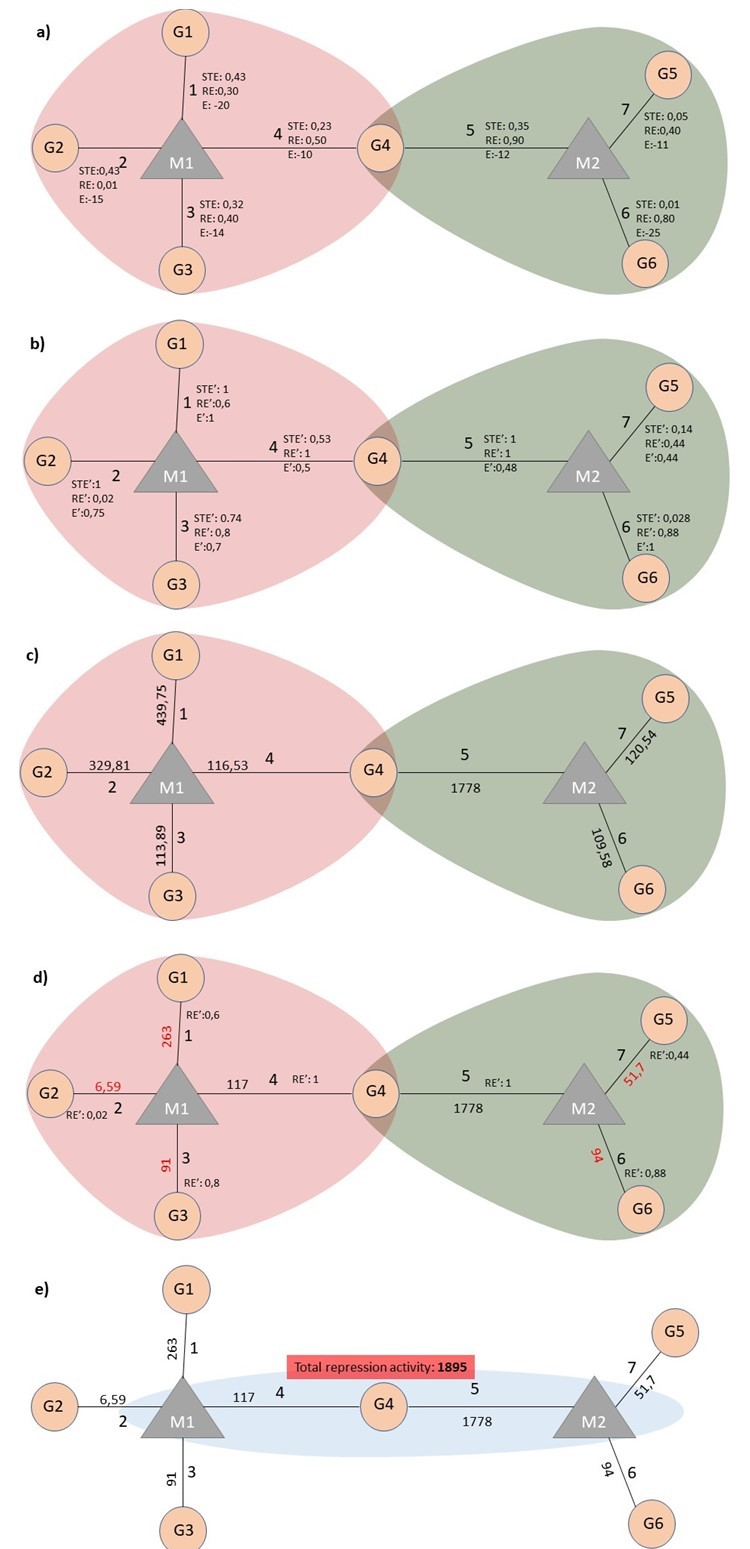
\includegraphics{fig2.jpg}
\caption{Calculations to determine of miRNA binding and repression
efficiency. \(G\), Gene; \(M\), miRNA; \(STE\), seed type effect;
\(RE\), Region Effect; \(E\), Energy; \(STE^\prime\), normalized values
of seed type efficiency coefficient; \(RE^\prime\), normalized values of
region efficiency coefficient; \(E^\prime\), normalized values of energy
coefficient.}\label{fig2}
}
\end{figure}

\iffalse

\%\% (\#TODO the equation is not considering binding factors, right?. We
should explain the calculation made in simulate function here, in simple
sentences. the function looks like this: \%\%
input\_graph\%\textgreater{}\% \%\%
tidygraph::activate(edges)\%\textgreater{}\% \%\%
group\_by(to)\%\textgreater{}\% \%\% mutate(mirna\_count\_per\_comp =
mirna\_count\_current\emph{comp\_count\_current}afff\_factor/sum(comp\_count\_current\emph{afff\_factor),
mirna\_count\_per\_comp = ifelse(is.na(mirna\_count\_per\_comp), 0,
mirna\_count\_per\_comp))\%\textgreater{}\% \%\%
ungroup()\%\textgreater{}\% \%\% mutate(effect\_pre = effect\_current,
effect\_current =
mirna\_count\_per\_comp}degg\_factor)\%\textgreater{}\% \%\%
group\_by(from)\%\textgreater{}\% \%\% mutate(comp\_count\_pre =
ifelse(comp\_count\_current\textless{} 0, 1, comp\_count\_current),
comp\_count\_current = comp\_count\_pre -
(sum(effect\_current)-sum(effect\_pre)), comp\_count\_current =
ifelse(comp\_count\_current\textless{} 0, 1,
comp\_count\_current))\%\textgreater{}\% \%\%
ungroup()\%\textgreater{}\% \%\% mutate(comp\_count\_list =
pmap(list(comp\_count\_list, comp\_count\_current), c), effect\_list =
pmap(list(effect\_list, effect\_current), c), mirna\_count\_list =
pmap(list(mirna\_count\_list, mirna\_count\_current), c)) \%\% ) \fi

I shown in figure and explained at following. I didn't fully understand
whether it is enough or not.

After miRNA binds to its target, but might not repress to bound target.
The functionality of bound miRNA on target depends on efficiency factors
like region that is binding sequence of miRNA on its target. Exact
repression efficiency of miRNA is calculated according to equation
\eqref{eq:4} (\autoref{fig2}d); \(RE^\prime_{gi}\), normalized values of
region efficiency coefficient between miRNA and gene. The cooperative
repression activity of miRNAs to their common targets is figured out as
shown in \autoref{fig2}e.

\hypertarget{breast-cancer-patient-dataset}{%
\subsubsection{Breast cancer patient
dataset}\label{breast-cancer-patient-dataset}}

We have applied our model in a real dataset for which experimental
measurements of various factors were available. Expression levels of
miRNA and genes in tumor and normal tissue of single patient are
retrieved from The Cancer Genome Atlas
\href{https://www.cancer.gov/about-nci/organization/ccg/research/structural-genomics/tcga}{TCGA}(\#TODO).
High-throughput experimental datasets which are provided miRNA:gene
target pairs with interaction factors (Helwak et al.
\protect\hyperlink{ref-helwak_mapping_2013}{2013}; Moore et al.
\protect\hyperlink{ref-moore_mirnatarget_2015}{2015}). We have combined
miRNA and gene expression datasets via miRNA:target gene dataset
retrieved from \ldots{} (\#FIX name of database and its citation)
answer-\textgreater{}suplementary datasets of (Helwak et al.
\protect\hyperlink{ref-helwak_mapping_2013}{2013}; Moore et al.
\protect\hyperlink{ref-moore_mirnatarget_2015}{2015}). Detailed
description of network construction and its code is available in
Supplementary data (\#TODO burada link nasıl olacak, word dosyası veya
PDF dosyası ismi mi vermemiz mi gerekiyor, yoksa sadece Sup Data
denilmesi yeterli mi? ilgili dosya: TCGA\_E9-A1N5\_article.Rmd). ABCC1
gene, over-expressed in tumor tissue, was selected as trigger for
simulation of integrated dataset. After simulation of network, we have
compared simulation results and tumor tissue expression levels.

\hypertarget{results-and-conclusions}{%
\subsection{Results and Conclusions}\label{results-and-conclusions}}

\hypertarget{networks-with-single-factor}{%
\subsubsection{Networks with single
factor}\label{networks-with-single-factor}}

We have developed a network-based approach to assess effects of
expression level changes in competitive ceRNA regulation. The basic mode
of miRNA repression activity has been based on miRNA and target
abundance in various researches (Arvey et al.
\protect\hyperlink{ref-arvey_target_2010}{2010}; Denzler et al.
\protect\hyperlink{ref-denzler_assessing_2014}{2014}). Our approach can
effortlessly calculate effects of expression changes when abundance
levels of miRNAs and targets is only available factor. In sample network
given in Figure (\autoref{fig1}), after an increase in expression level
of a gene (G2), expression values of other genes also changed due to
redistribution of miRNA among its targets. Previous studies have shown
that if a gene abundance increases in ceRNA system, expression levels of
genes targeted by shared miRNA are also affected (Lai, Wolkenhauer, and
Vera \protect\hyperlink{ref-lai_understanding_2016}{2016}; Salmena et
al. \protect\hyperlink{ref-salmena_cerna_2011}{2011}; Tay, Rinn, and
Pandolfi \protect\hyperlink{ref-tay_multilayered_2014}{2014}). It was
observed that expression levels of primary neighborhoods which do not
interact with another miRNA of the trigger gene change in relation to
their expression. However, expression level change of common target (G4)
in network has been observed different from G1 that has the same
expression value with G4 target at initial conditions because more than
one miRNA repress this target (\autoref{fig1}d) (\#FIX last sentence
needs some clarification, after ``but cooperative\ldots{}'').

Genes targeted by multiple miRNAs act as a trigger for adjacent local
neighborhood of targeting miRNAs, causing changes in expression levels
of genes outside the local neighborhood of original trigger gene.
Therefore, primary expression level change in gene (G2) causes changes
in other group of genes (G5 and G6) even though original trigger gene
(G2) and genes in other group are not targeted by common miRNA. In
addition, as shown by ceRNA hypothesis model of Ala et al., after the
increase of gene expression level of G2, the miRNA that is found in the
same group (M1) tended to be less repressive on its remaining targets
(G1, G3 and G4). It's important to note that the changes in gene
expression levels will have more pronounced effect if miRNA:target ratio
is high, i.e., more miRNA available per target, which was reported in
previous findings (Arvey et al.
\protect\hyperlink{ref-arvey_target_2010}{2010}; Bosson, Zamudio, and
Sharp \protect\hyperlink{ref-bosson_endogenous_2014}{2014}; Denzler et
al. \protect\hyperlink{ref-denzler_assessing_2014}{2014}). \href{}{}

\begin{figure}
\hypertarget{fig3}{%
\centering
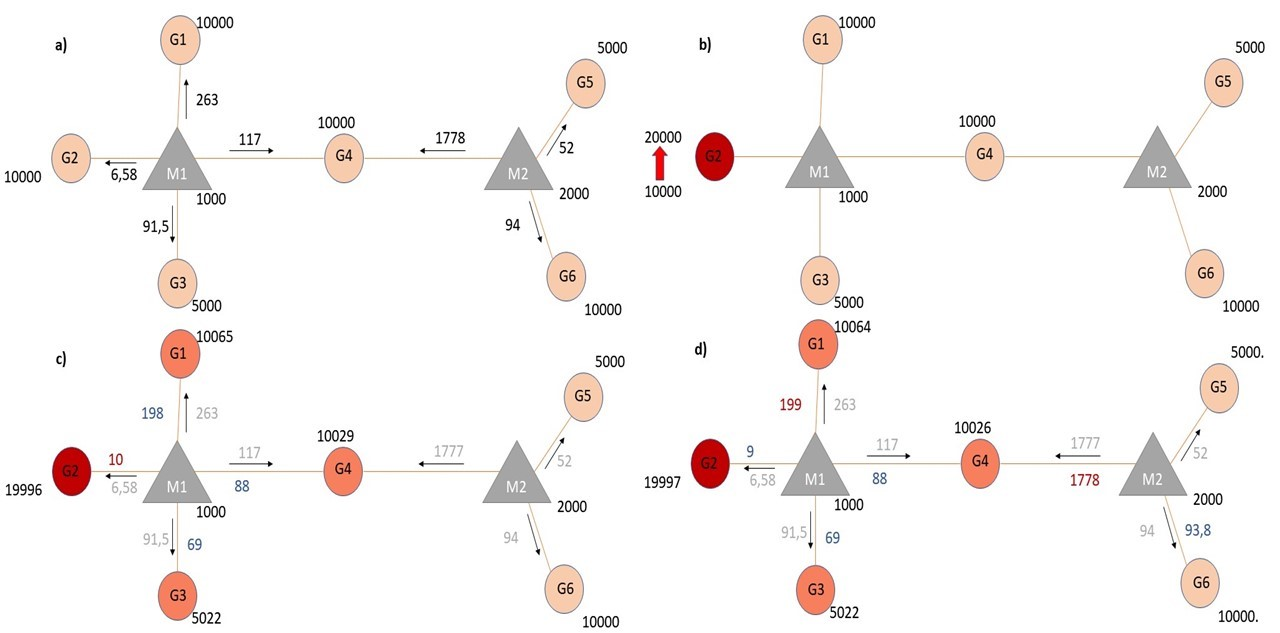
\includegraphics{Fig3.jpg}
\caption{Target regulations with interaction parameters. a) In the
steady-state the repression activity of miRNAs on the targets after
binding and repression efficiency. b) The changes the repression
activities after increasing of G2 expression. c) Perturbation of primary
neighborhoods of M1 miRNA (M1 miRNA group). d) Regulation of gene
expression of other gene group via triggering target (common target
between M1 and M2).}\label{fig3}
}
\end{figure}

\hypertarget{competing-endogenous-rnatarget-networks-based-on-interaction-factors}{%
\subsubsection{Competing Endogenous RNA:Target networks based on
interaction
factors}\label{competing-endogenous-rnatarget-networks-based-on-interaction-factors}}

\href{}{\#FIX}: \textless{}\textgreater{} ``title should be more
informative''-\textgreater{} answer.

Earlier studies reported that miRNA regulatory interactions are affected
by different parameters. For example, Xu et al.~have investigated the
importance of seed pairing type between miRNAs and their targets and
target site location by using proteomics dataset (Xu, Wang, and Liu
\protect\hyperlink{ref-xu_characterization_2014}{2014}). They have
proposed that the features of binding between miRNA and target can be
critical for miRNA efficiency. In addition, binding energy between miRNA
and targets is a significant determinant for miRNA efficiency and it has
been reported that strength of miRNA:target interactions is depended on
binding energy of complexes (Breda et al.
\protect\hyperlink{ref-breda_quantifying_2015}{2015}). Similarly,
another study revealed that affinity is correlated with seed pairing of
miRNA:target pairs and suggested that affinity is correlated with number
of canonical seed base pairing (Bosson, Zamudio, and Sharp
\protect\hyperlink{ref-bosson_endogenous_2014}{2014}). Therefore, we
have integrated aforementioned interaction parameters that could be
useful for predicting miRNA repression activity more accurately. The
sample dataset used in \autoref{fig1} is recalculated with additional
factors \autoref{tab:one} in effect with same trigger, two fold increase
in Gene2 (\autoref{fig3}). When the factors were taken into account in
the system, miRNA efficiencies varied as shown in \autoref{fig3}a.
Although the miRNA:target expression ratios in steady-state were same in
comparison with the sample dataset without factors, efficiency of
binding and repression have changed.

It is considered that entire miRNAs in the system affect targets
according to target:total target ratio \autoref{fig1}a, when interaction
factors did not take into account. However, in presence of interaction
factors in miRNA:target interaction network (shown in
\autoref{tab:one}), miRNAs are distributed according to target:total
target ratio and affinity factors in first like shown in
\autoref{fig2}c.~After affinity mediated propotional distribution of
miRNA expression, degradation factor is considered to specify count of
repressive miRNA in pairs because entire bound miRNA target pairs might
not be resulted with degradation (It is figured out shown in
\autoref{fig2}d). For this reason, miRNA1 (M1) has more weak repressive
effect (shown as edge variables) on target Gene2 \autoref{fig3}a in
comparison with miRNA1 (M1):Gene2 (G2) interaction in \autoref{fig1}a.
On the other hand, it is possible that taking into accont of these
interaction factors could cause increasing miRNA repression activity
like in miRNA2:Gene4 interaction \autoref{fig3}a. When expression of
Gene2 (G2) increased, expression values of all genes also changed
differentially because of contribution of efficiency factors
(\autoref{fig3} b,c,d). We have considered that in our approach energy
and seed type of pairs is significant for binding and targeted region is
important for repression.

\begin{table}[ht]
\centering
\caption{Expression values of elements and interaction factors of miRNA:target interactions in \autoref{fig3}} 
\begin{tabular}{rllrrrrr}
  \hline
 & competing & miRNA & Competing expression & miRNA expression & seed type & region & energy \\ 
  \hline
   & Gene1 & Mir1 & 10000.00 & 1000.00 & 0.43 & 0.30 & -20.00 \\ 
   & Gene2 & Mir1 & 10000.00 & 1000.00 & 0.43 & 0.01 & -15.00 \\ 
   & Gene3 & Mir1 & 5000.00 & 1000.00 & 0.32 & 0.40 & -14.00 \\ 
   & Gene4 & Mir1 & 10000.00 & 1000.00 & 0.23 & 0.50 & -10.00 \\ 
   & Gene4 & Mir2 & 10000.00 & 2000.00 & 0.35 & 0.90 & -12.00 \\ 
   & Gene5 & Mir2 & 5000.00 & 2000.00 & 0.05 & 0.40 & -11.00 \\ 
   & Gene6 & Mir2 & 10000.00 & 2000.00 & 0.01 & 0.80 & -25.00 \\ 
   \hline
\end{tabular}
\label{tab:one}
\end{table}

In regulation of miRNA target sample system (\autoref{fig3}), miRNA (M1)
repressive efficiency on the primary triggering gene (G2) is low in
steady-state. So it has been observed that the regulatory activities of
miRNA on the targets are weak after the increase of miRNA target G2.
When model is triggered with two fold increase in expression level of
common target (G4), the changes of other gene expressions have observed
more prominent \href{}{}. Furthermore, change in expression level of
target gene that has strong miRNA repression efficiency resulted in
evident perturbation in network. On the other hand, it was observed that
Gene2 was weakly affected from change of Gene4 expression because of its
weak interaction factors. Since perturbation efficiency of each gene is
different, we have developed a function which screens each gene in the
network for their perturbation efficiencies. \textbf{(see details in
Supplementary File(fig1\_2app.Rmd)}. On the other hand, when we applied
the method on the minimal dataset, Gene4 has been found to be the most
efficient element in terms of number of perturbed elements and miRNA2
(M2) has been found to be causing the highest mean in expression
changes. {[}{]}{[}\#TODO2{]}

We used our model to simulate a real dataset which contains thousands of
genes and hundreds of miRNAs. Our model can successfully simulate
perturbations in such large network despite complex behaviors and
struggle to reach steady-state \textbf{(see details in Supplementary
File(TCGA\_E9-A1N5\_article.Rmd)}. Simulations show that change in
expression level of single gene has potential to effect whole network,
perturbing almost all nodes. These observations are in accordance with
competing endogenous RNA hypothesis where genes targeted with many
common miRNAs subsequently transmit perturbation to neighboring groups.

Network based approaches for analyzing miRNA:target interactions have
been developed in earlier studies. An initial attempt demonstrated the
ceRNA crosstalk in a network-like minimal interaction structure with
concentrations of ceRNA and miRNAs (Figliuzzi, Marinari, and De Martino
\protect\hyperlink{ref-figliuzzi_micrornas_2013}{2013}). Next, a network
based kinetic model integrating miRNA and target rates of transcription,
degradation, binding and unbinding was developed (Nitzan et al.
\protect\hyperlink{ref-nitzan_interactions_2014}{2014}) using high
throughput experimental dataset about miR-92a depletion (Helwak et al.
\protect\hyperlink{ref-helwak_mapping_2013}{2013}). It was demonstrated
that distant ceRNAs can interact with each other via indirect links, and
the interactions are effected depending on distance between ceRNAs or
topological features of network (Nitzan et al.
\protect\hyperlink{ref-nitzan_interactions_2014}{2014}). More recently,
an approach to detect ceRNA interaction by using the miRNA expression,
gene expression and common miRNAs between gene targets was developed
(Markus List \protect\hyperlink{ref-markus_list_sponge_2017}{2017})
which was effective in analyzing genes through miRNAs. Based on the
observations that a miRNA can exhibit strong functionality to a target
but may not against an other, the authors have concluded that existing
miRNA based approach may not be suitable for understanding regulations
of ceRNA interactions.

{[}\#Add{]}More recently, Silveira et al.~have developed miRmapper
package for using with R programme (Silveira et al.
\protect\hyperlink{ref-da2018mirmapper}{2018}). Researchers have
utilized the adjacency matrix to associate miRNAs using differentially
expressed genes and found similarities of miRNAs with this approach.
Authors who utilized the approach in dataset of bladder cancer cell line
have identified significant miRNAs in network, and miRNAs which work
synergistically.

{[}\#Add{]} Today, there are many of tools that provide predicted or
experimentally validated miRNA:target interaction dataset. The datasets
that contain weak, proteomic analysis like western blot, and strong,
crosslinking and immunoprecipitation CLiP, experimentally evidence are
more reliable sources than prediction datasets. While in experimentally
weak supported datasets it is not known that indirect or direct target
of miRNAs in cell, high-throughput methods ensure handling of AGO
(Argounate Protein) interacted miRNAs. For this reason we have preferred
to utilize high-throughput datasets in our application. Especially, we
collected datasets that depend on chimeric (Helwak et al.
\protect\hyperlink{ref-helwak_mapping_2013}{2013}; Moore et al.
\protect\hyperlink{ref-moore_mirnatarget_2015}{2015}) reading of miRNA:
target pairs from among these datasets because they contain exact
complementary seed regions.

{[}\#Add{]} Although these experimental sources include exact binding
sites, they do not provides which miRNA is functional or not (Liu and
Wang \protect\hyperlink{ref-liu2019prediction}{2019}). We have used the
features of bound miRNA:target pairs and scaled these parameters inside
groups that is consisted according to, ceRNA (Competing Endogenous RNA),
genes targeted by the same miRNA. In scaling process, we specified the
interaction factors as numeric values in accordance with previous
studies. Energy values in miRNA:target pairs are represented by
high-throughput studies (Helwak et al.
\protect\hyperlink{ref-helwak_mapping_2013}{2013}; Moore et al.
\protect\hyperlink{ref-moore_mirnatarget_2015}{2015}) which are utilized
in this study. On the other hand, we have specified the other
interaction factors, seed type and location of binding region on the
target, as numeric values based on the previous studies.(Grimson et al.
\protect\hyperlink{ref-grimson_microrna_2007}{2007}) have compared the
seed types' effect on target repression with few miRNA had canonical
seed pairing in their study. Additionally, (Bartel
\protect\hyperlink{ref-bartel_micrornas:_2009}{2009}) and (Betel et al.
\protect\hyperlink{ref-betel2010comprehensive}{2010}) have studied on
functional and non-functional seed interactions. Based on results of
these studies we have arranged seed types of miRNA:target interactions
as numeric values. We also have redefined location of binding region on
the target as numeric values, based on studies of (Hausser et al.
\protect\hyperlink{ref-hausser_analysis_2013}{2013}) and (Helwak et al.
\protect\hyperlink{ref-helwak_mapping_2013}{2013}). With this process,
we have handled this entegrated dataset in context of competitor
behaviours and functionality of interactions.

{[}\#Add{]}The main advantage of the method, ceRNAnetsim package, is
providing various functions which contain optionally arguments. So,
users can run the functions in accordance with their own data. For
example, the functions can work without interaction factors or with a
simple interaction factor that is specified by user. Furthermore, it can
also be operated according to a different parameter(s) provided by the
user.In this study, we have preferred to run model, shown in
\emph{Multifactorial calculations in miRNA:target network} section.

{[}\#TODO answer{]} We have observed that the results of simulation with
ABCC1 gene, \emph{Multidrug resistance-associated protein 1}, which is
one of the most significant factor to develop resistance against
chemotherapotic agents(Atalay, Demirkazik, and Gunduz
\protect\hyperlink{ref-atalay2008role}{2008}; Lu et al.
\protect\hyperlink{ref-lu2015microrna}{2015}; Atalay et al.
\protect\hyperlink{ref-atalay2006multidrug}{2006}) is not convenient
with tumor tissue expression values, when we compared the tumor gene
expression dataset retrieved from
\href{https://www.cancer.gov/about-nci/organization/ccg/research/structural-genomics/tcga}{TCGA}
and simulation results obtained via our approach. Simulation results
were not expected to be consistent with tumor tissue expression values
because large number of abnormal regulations were observed in these
tissues. So, it might not said that a single gene is responsible for
entire regulations in cancer cells. Besides, the all other factors such
as up/down regulation of miRNAs or other genes were ignored. Therefore,
it would be more useful to test our approach with an ideal dataset that
includes entire informations of gene expression values before and after
the regulation of a known gene at existing tissue, and miRNA expression
values of this tissue at initial conditions.

In our approach, we have not taken into account transcription,
degradation or binding rates of elements in network. Because, although
it is known as the miRNAs are highly stable, the transcription and
degradation rates of miRNAs change depending on cellular conditions
(Rüegger and Großhans
\protect\hyperlink{ref-ruegger_microrna_2012}{2012}). However, due to
lack of datasets including degradation and transcription rates of miRNAs
at specific cellular conditions, such factors are neglected in our
model. Additionally, other regulation parameters such as gene-gene
interactions and transcription factors are ignored but the network
structure is flexible and can integrate additional regulation elements
as they become available. In the future, with developments in
experimental techniques about miRNAs:target interaction dynamica, more
accurate results can be obtained from our model resulting in better
understanding and predictions of abnormal regulations and pathways
underlying diseases or conditions.

\hypertarget{references}{%
\subsection*{References}\label{references}}
\addcontentsline{toc}{subsection}{References}

\hypertarget{refs}{}
\leavevmode\hypertarget{ref-ala_integrated_2013}{}%
Ala, U., F. A. Karreth, C. Bosia, A. Pagnani, R. Taulli, V. Leopold, Y.
Tay, P. Provero, R. Zecchina, and P. P. Pandolfi. 2013. ``Integrated
Transcriptional and Competitive Endogenous RNA Networks Are
Cross-Regulated in Permissive Molecular Environments.''
\emph{Proceedings of the National Academy of Sciences} 110 (18):
7154--9. \url{https://doi.org/10.1073/pnas.1222509110}.

\leavevmode\hypertarget{ref-arvey_target_2010}{}%
Arvey, Aaron, Erik Larsson, Chris Sander, Christina S Leslie, and Debora
S Marks. 2010. ``Target mRNA Abundance Dilutes microRNA and siRNA
Activity.'' \emph{Molecular Systems Biology} 6 (April).
\url{https://doi.org/10.1038/msb.2010.24}.

\leavevmode\hypertarget{ref-atalay2006multidrug}{}%
Atalay, Can, Ismet Deliloglu Gurhan, Cigdem Irkkan, and Ufuk Gunduz.
2006. ``Multidrug Resistance in Locally Advanced Breast Cancer.''
\emph{Tumor Biology} 27 (6): 309--18.

\leavevmode\hypertarget{ref-atalay2008role}{}%
Atalay, C, A Demirkazik, and U Gunduz. 2008. ``Role of Abcb1 and Abcc1
Gene Induction on Survival in Locally Advanced Breast Cancer.''
\emph{Journal of Chemotherapy} 20 (6): 734--39.

\leavevmode\hypertarget{ref-bartel_micrornas_2004}{}%
Bartel, David P. 2004. ``MicroRNAs.'' \emph{Cell} 116 (2): 281--97.
\url{https://doi.org/10.1016/S0092-8674(04)00045-5}.

\leavevmode\hypertarget{ref-bartel_micrornas:_2009}{}%
Bartel, David P. 2009. ``MicroRNAs: Target Recognition and Regulatory
Functions.'' \emph{Cell} 136 (2): 215--33.
\url{https://doi.org/10.1016/j.cell.2009.01.002}.

\leavevmode\hypertarget{ref-betel2010comprehensive}{}%
Betel, Doron, Anjali Koppal, Phaedra Agius, Chris Sander, and Christina
Leslie. 2010. ``Comprehensive Modeling of microRNA Targets Predicts
Functional Non-Conserved and Non-Canonical Sites.'' \emph{Genome
Biology} 11 (8): R90.

\leavevmode\hypertarget{ref-bosson_endogenous_2014}{}%
Bosson, Andrew D., Jesse R. Zamudio, and Phillip A. Sharp. 2014.
``Endogenous miRNA and Target Concentrations Determine Susceptibility to
Potential ceRNA Competition.'' \emph{Molecular Cell} 56 (3): 347--59.
\url{https://doi.org/10.1016/j.molcel.2014.09.018}.

\leavevmode\hypertarget{ref-breda_quantifying_2015}{}%
Breda, Jeremie, Andrzej J. Rzepiela, Rafal Gumienny, Erik van Nimwegen,
and Mihaela Zavolan. 2015. ``Quantifying the Strength of miRNA--Target
Interactions.'' \emph{Methods} 85 (September): 90--99.
\url{https://doi.org/10.1016/j.ymeth.2015.04.012}.

\leavevmode\hypertarget{ref-cao_predicting_2012}{}%
Cao, Song, and Shi-Jie Chen. 2012. ``Predicting Kissing Interactions in
microRNA--Target Complex and Assessment of microRNA Activity.''
\emph{Nucleic Acids Research} 40 (10): 4681--90.
\url{https://doi.org/10.1093/nar/gks052}.

\leavevmode\hypertarget{ref-cesana_deciphering_2013}{}%
Cesana, Marcella, and George Q. Daley. 2013. ``Deciphering the Rules of
ceRNA Networks.'' \emph{Proceedings of the National Academy of Sciences
of the United States of America} 110 (18): 7112--3.
\url{https://doi.org/10.1073/pnas.1305322110}.

\leavevmode\hypertarget{ref-chi2012alternative}{}%
Chi, Sung Wook, Gregory J Hannon, and Robert B Darnell. 2012. ``An
Alternative Mode of microRNA Target Recognition.'' \emph{Nature
Structural \& Molecular Biology} 19 (3): 321.

\leavevmode\hypertarget{ref-denzler_assessing_2014}{}%
Denzler, Rémy, Vikram Agarwal, Joanna Stefano, David P. Bartel, and
Markus Stoffel. 2014. ``Assessing the ceRNA Hypothesis with Quantitative
Measurements of miRNA and Target Abundance.'' \emph{Molecular Cell} 54
(5): 766--76. \url{https://doi.org/10.1016/j.molcel.2014.03.045}.

\leavevmode\hypertarget{ref-denzler_impact_2016}{}%
Denzler, Rémy, Sean E. McGeary, Alexandra C. Title, Vikram Agarwal,
David P. Bartel, and Markus Stoffel. 2016. ``Impact of MicroRNA Levels,
Target-Site Complementarity, and Cooperativity on Competing Endogenous
RNA-Regulated Gene Expression.'' \emph{Molecular Cell} 64 (3): 565--79.
\url{https://doi.org/10.1016/j.molcel.2016.09.027}.

\leavevmode\hypertarget{ref-figliuzzi_micrornas_2013}{}%
Figliuzzi, Matteo, Enzo Marinari, and Andrea De Martino. 2013.
``MicroRNAs as a Selective Channel of Communication Between Competing
RNAs: A Steady-State Theory.'' \emph{Biophysical Journal} 104 (5):
1203--13. \url{https://doi.org/10.1016/j.bpj.2013.01.012}.

\leavevmode\hypertarget{ref-grimson_microrna_2007}{}%
Grimson, Andrew, Kyle Kai-How Farh, Wendy K. Johnston, Philip
Garrett-Engele, Lee P. Lim, and David P. Bartel. 2007. ``MicroRNA
Targeting Specificity in Mammals: Determinants Beyond Seed Pairing.''
\emph{Molecular Cell} 27 (1): 91--105.
\url{https://doi.org/10.1016/j.molcel.2007.06.017}.

\leavevmode\hypertarget{ref-hafner_transcriptome-wide_2010}{}%
Hafner, Markus, Markus Landthaler, Lukas Burger, Mohsen Khorshid, Jean
Hausser, Philipp Berninger, Andrea Rothballer, et al. 2010.
``Transcriptome-Wide Identification of RNA-Binding Protein and MicroRNA
Target Sites by PAR-CLIP.'' \emph{Cell} 141 (1): 129--41.
\url{https://doi.org/10.1016/j.cell.2010.03.009}.

\leavevmode\hypertarget{ref-hausser_analysis_2013}{}%
Hausser, J., A. P. Syed, B. Bilen, and M. Zavolan. 2013. ``Analysis of
CDS-Located miRNA Target Sites Suggests That They Can Effectively
Inhibit Translation.'' \emph{Genome Research} 23 (4): 604--15.
\url{https://doi.org/10.1101/gr.139758.112}.

\leavevmode\hypertarget{ref-helwak_mapping_2013}{}%
Helwak, Aleksandra, Grzegorz Kudla, Tatiana Dudnakova, and David
Tollervey. 2013. ``Mapping the Human miRNA Interactome by CLASH Reveals
Frequent Noncanonical Binding.'' \emph{Cell} 153 (3): 654--65.
\url{https://doi.org/10.1016/j.cell.2013.03.043}.

\leavevmode\hypertarget{ref-lai_understanding_2016}{}%
Lai, Xin, Olaf Wolkenhauer, and Julio Vera. 2016. ``Understanding
microRNA-Mediated Gene Regulatory Networks Through Mathematical
Modelling.'' \emph{Nucleic Acids Research} 44 (13): 6019--35.
\url{https://doi.org/10.1093/nar/gkw550}.

\leavevmode\hypertarget{ref-lewis_conserved_2005}{}%
Lewis, Benjamin P., Christopher B. Burge, and David P. Bartel. 2005.
``Conserved Seed Pairing, Often Flanked by Adenosines, Indicates That
Thousands of Human Genes Are MicroRNA Targets.'' \emph{Cell} 120 (1):
15--20. \url{https://doi.org/10.1016/j.cell.2004.12.035}.

\leavevmode\hypertarget{ref-liu2019prediction}{}%
Liu, Weijun, and Xiaowei Wang. 2019. ``Prediction of Functional microRNA
Targets by Integrative Modeling of microRNA Binding and Target
Expression Data.'' \emph{Genome Biology} 20 (1): 18.

\leavevmode\hypertarget{ref-lu2015microrna}{}%
Lu, Lin, Fang Ju, Hui Zhao, and Xuezhen Ma. 2015. ``MicroRNA-134
Modulates Resistance to Doxorubicin in Human Breast Cancer Cells by
Downregulating Abcc1.'' \emph{Biotechnology Letters} 37 (12): 2387--94.

\leavevmode\hypertarget{ref-markus_list_sponge_2017}{}%
Markus List, Marcel Schulz. 2017. ``SPONGE.'' Bioconductor.
\url{https://doi.org/10.18129/B9.bioc.SPONGE}.

\leavevmode\hypertarget{ref-moore_mirnatarget_2015}{}%
Moore, Michael J., Troels K. H. Scheel, Joseph M. Luna, Christopher Y.
Park, John J. Fak, Eiko Nishiuchi, Charles M. Rice, and Robert B.
Darnell. 2015. ``miRNA-Target Chimeras Reveal miRNA 3'-End Pairing as a
Major Determinant of Argonaute Target Specificity.'' \emph{Nature
Communications} 6 (November): 8864.
\url{https://doi.org/10.1038/ncomms9864}.

\leavevmode\hypertarget{ref-nitzan_interactions_2014}{}%
Nitzan, Mor, Avital Steiman-Shimony, Yael Altuvia, Ofer Biham, and Hanah
Margalit. 2014. ``Interactions Between Distant ceRNAs in Regulatory
Networks.'' \emph{Biophysical Journal} 106 (10): 2254--66.
\url{https://doi.org/10.1016/j.bpj.2014.03.040}.

\leavevmode\hypertarget{ref-robinson_modelling_2018}{}%
Robinson, J. M., and W. A. Henderson. 2018. ``Modelling the Structure of
a ceRNA-Theoretical, Bipartite microRNA-mRNA Interaction Network
Regulating Intestinal Epithelial Cellular Pathways Using R
Programming.'' \emph{BMC Research Notes} 11 (1): 19.
\url{https://doi.org/10.1186/s13104-018-3126-y}.

\leavevmode\hypertarget{ref-ruegger_microrna_2012}{}%
Rüegger, Stefan, and Helge Großhans. 2012. ``MicroRNA Turnover: When,
How, and Why.'' \emph{Trends in Biochemical Sciences} 37 (10): 436--46.
\url{https://doi.org/10.1016/j.tibs.2012.07.002}.

\leavevmode\hypertarget{ref-salmena_cerna_2011}{}%
Salmena, Leonardo, Laura Poliseno, Yvonne Tay, Lev Kats, and Pier Paolo
Pandolfi. 2011. ``A ceRNA Hypothesis: The Rosetta Stone of a Hidden RNA
Language?'' \emph{Cell} 146 (3): 353--58.
\url{https://doi.org/10.1016/j.cell.2011.07.014}.

\leavevmode\hypertarget{ref-da2018mirmapper}{}%
Silveira, Willian da, Ludivine Renaud, Jonathan Simpson, William Glen,
Edward Hazard, Dongjun Chung, and Gary Hardiman. 2018. ``MiRmapper: A
Tool for Interpretation of miRNA--mRNA Interaction Networks.''
\emph{Genes} 9 (9): 458.

\leavevmode\hypertarget{ref-tay_multilayered_2014}{}%
Tay, Yvonne, John Rinn, and Pier Paolo Pandolfi. 2014. ``The
Multilayered Complexity of ceRNA Crosstalk and Competition.''
\emph{Nature} 505 (7483): 344--52.
\url{https://doi.org/10.1038/nature12986}.

\leavevmode\hypertarget{ref-werfel_preferential_2017}{}%
Werfel, Stanislas, Simon Leierseder, Benjamin Ruprecht, Bernhard Kuster,
and Stefan Engelhardt. 2017. ``Preferential microRNA Targeting Revealed
by in Vivo Competitive Binding and Differential Argonaute
Immunoprecipitation.'' \emph{Nucleic Acids Research} 45 (17): 10218--28.
\url{https://doi.org/10.1093/nar/gkx640}.

\leavevmode\hypertarget{ref-xu_characterization_2014}{}%
Xu, Wenlong, Zixing Wang, and Yin Liu. 2014. ``The Characterization of
microRNA-Mediated Gene Regulation as Impacted by Both Target Site
Location and Seed Match Type.'' Edited by Thomas Preiss. \emph{PLoS ONE}
9 (9): e108260. \url{https://doi.org/10.1371/journal.pone.0108260}.


\end{document}
